% Author: Izaak Neutelings (December 2020)
\documentclass[border=3pt,tikz]{standalone}
\usepackage{amsmath}
\usepackage{etoolbox} % ifthen
\usepackage{tikz}
\usetikzlibrary{arrows.meta} % for arrow size
\tikzset{>=latex} % for LaTeX arrow head

\colorlet{xcol}{blue!70!black}
\colorlet{vcol}{green!60!black}
\colorlet{myred}{red!80!black}
\colorlet{myblue}{blue!80!black}
\colorlet{mypurple}{blue!50!red!80}
\colorlet{metalcol}{blue!25!black!30!white}
\tikzstyle{vvec}=[->,vcol,very thick,line cap=round]
\tikzstyle{node}=[xcol,scale=0.8]
\tikzstyle{metal}=[draw=metalcol!10!black,rounded corners=0.1,
  top color=metalcol,bottom color=metalcol!80!black,shading angle=10]
\tikzstyle{ring}=[metalcol!20!black,double=metalcol!70!black,double distance=1.2,line width=0.3]
\tikzstyle{rope}=[brown!20!black,double=brown!70!black,
  double distance=1.2,line width=0.6] %very thick,line cap=round
\tikzstyle{wood}=[draw=brown!80!black,rounded corners=0.1,
  top color=brown!80,bottom color=brown!80!black!80,shading angle=10]
\def\tick#1#2{\draw[thick] (#1) ++ (#2:0.1) --++ (#2-180:0.2)}
\tikzstyle{myarr}=[-{Latex[length=3,width=2]},vcol!40]
\tikzstyle{mydoublearr}=[{Latex[length=3,width=2]}-{Latex[length=3,width=2]},vcol!40]

\begin{document}

% SUM TRAVELING WAVE = STANDING WAVE
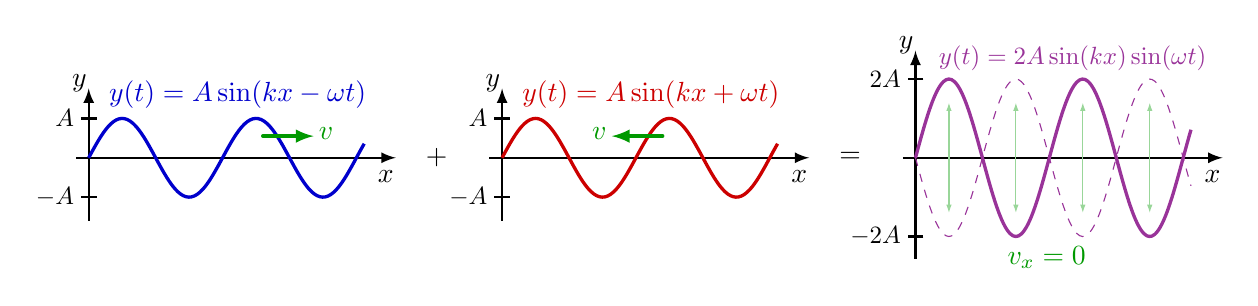
\begin{tikzpicture}
  \def\xmax{3.5}
  \def\ymax{0.80}
  \def\A{0.50}      % amplitude
  \def\lam{1.7}     % wavelength
  \def\s{1.5*\xmax} % shift
  
  % RIGHT-TRAVELING
  \draw[->,thick] (-0.2*\ymax,0) -- (0.4+\xmax,0) node[right=4,below left=1] {$x$};
  \draw[->,thick] (0,-\ymax) -- (0,1.1*\ymax) node[below=2,above left=-3] {$y$};
  \tick{0,\A}{0} node[scale=0.9,left=-1] {$A$};
  \tick{0,-\A}{0} node[scale=0.9,left=-1] {$-A$};
  \draw[myblue,very thick,samples=100,smooth,variable=\x,domain=0:\xmax]
    plot(\x,{\A*sin(360/\lam*\x)});
  \draw[vvec] (1.3*\lam,0.55*\A) --++ (0.38*\lam,0) node[above=1,right=-2] {$v$};
  \node[above,myblue] at (0.54*\xmax,\A) {$y(t)=A\sin(kx-\omega t)$};
  \node at ({0.505*(\xmax+\s)},0) {$+$};
  
  % LEFT-TRAVELING
  \begin{scope}[shift={(\s,0)}]
    \draw[->,thick] (-0.2*\ymax,0) -- (0.4+\xmax,0) node[right=4,below left=1] {$x$};
    \draw[->,thick] (0,-\ymax) -- (0,1.1*\ymax) node[below=2,above left=-3] {$y$};
    \tick{0,\A}{0} node[scale=0.9,left=-1] {$A$};
    \tick{0,-\A}{0} node[scale=0.9,left=-1] {$-A$};
    \draw[myred,very thick,samples=100,smooth,variable=\x,domain=0:\xmax]
      plot(\x,{\A*sin(360/\lam*\x)});
    \draw[vvec] (1.2*\lam,0.55*\A) --++ (-0.38*\lam,0) node[above=1,left=-2] {$v$};
    \node[above,myred] at (0.54*\xmax,\A) {$y(t)=A\sin(kx+\omega t)$};
    \node at ({0.505*(\xmax+\s)},0) {$=$};
  \end{scope}
  
  % STANDING WAVE
  \begin{scope}[shift={(2*\s,0)}]
    \draw[->,thick] (-0.2*\ymax,0) -- (0.4+\xmax,0) node[right=4,below left=1] {$x$};
    \draw[->,thick] (0,-1.6*\ymax) -- (0,1.7*\ymax) node[below=2,above left=-3] {$y$};
    \tick{0,2*\A}{0} node[scale=0.9,left=-1] {$2A$};
    \tick{0,-2*\A}{0} node[scale=0.9,left=-1] {$-2A$};
    \draw[mypurple,very thick,samples=100,smooth,variable=\x,domain=0:\xmax]
      plot(\x,{2*\A*sin(360/\lam*\x)});
    \draw[mypurple,dashed,samples=100,smooth,variable=\x,domain=0:\xmax]
      plot(\x,{-2*\A*sin(360/\lam*\x)});
    \node[vcol,left=1,below=0] at (\lam,-2*\A) {$v_x=0$};
    \node[above,mypurple,scale=0.9] at (0.57*\xmax,2*\A) {$y(t)=2A\sin(kx)\sin(\omega t)$};
    \foreach \i in {1,...,4}{
      \draw[mydoublearr] ({2*\i-1)*\lam/4},1.4*\A) --++ (0,-2.8*\A);
    }
  \end{scope}
  
\end{tikzpicture}

% WAVE t = 0
\def\xmax{3.2}
\def\ymax{0.725}
\def\A{0.80*\ymax}   % amplitude
\def\lam{0.92*\xmax} % wavelength
\def\om{360/(\lam)}  % omega (degrees)
\def\s{3.1*\A}       % shift
\begin{tikzpicture}
  \def\wave#1#2{
    \draw[->,thick] (-0.2*\ymax,0) -- (1.1*\xmax,0) node[right=4,below left=1] {$x$};
    \draw[->,thick] (0,-\ymax) -- (0,1.2*\ymax); %node[below=2,above left=-3] {$y$};
    \draw[xcol,very thick,samples=100,smooth,variable=\x,domain=0:\xmax]
      plot(\x,{\A*sin(\om*\x)*cos(#1)});
    %\draw[myarr] (0.25*\lam,{ 0.85*\A*cos(#1)}) --++ (0,{-0.7*\A*cos(#1)});
    %\draw[myarr] (0.75*\lam,{-0.85*\A*cos(#1)}) --++ (0,{ 0.7*\A*cos(#1)});
    \tick{0,\A}{0} node[scale=0.9,left=-1] {$A$};
    \tick{0,-\A}{0} node[scale=0.9,left=-1] {$-A$};
    \tick{\lam/2,0}{90};
    \tick{\lam,0}{90}; %node[scale=0.9,right=1,below=5,fill=white,inner sep=1] {$\lambda$};
    \node[left,scale=0.9] at (-0.4*\ymax,0) {$t=#2$};
  }
  
  % t = 0
  \draw[dashed,blue!50!black!70]
    (0.5*\lam,0.25*\ymax) node[scale=0.9,right=4,above=-3] {$\strut\lambda/2$}
    --++ (0,-8*\s-0.8*\ymax);
  \draw[dashed,blue!50!black!70]
    (\lam,0.25*\ymax) node[scale=0.9,above=-3] {$\strut\lambda$}
    --++ (0,-8*\s-0.8*\ymax);
  \wave{0}{0}
  \node[below=2,above left=-3] at (0,1.2*\ymax) {$y$};
  
  % t = T/6
  \begin{scope}[shift={(0,-\s)}]
    \wave{60}{T/6}
    \draw[myarr] (0.25*\lam,{ 0.85*\A*cos(60)}) --++ (0,{-0.7*\A*cos(60)});
    \draw[myarr] (0.75*\lam,{-0.85*\A*cos(60)}) --++ (0,{ 0.7*\A*cos(60)});
  \end{scope}
  
  % t = T/4
  \begin{scope}[shift={(0,-2*\s)}]
    \wave{90}{T/4}
    %\tick{\lam,0}{90} node[scale=0.9,below right=-1] {$\lambda$};
    \draw[myarr] (0.25*\lam,{-0.10*\A}) --++ (0,{-0.7*\A});
    \draw[myarr] (0.75*\lam,{ 0.10*\A}) --++ (0,{ 0.7*\A});
  \end{scope}
  
  % t = T/3
  \begin{scope}[shift={(0,-3*\s)}]
    \wave{120}{T/3}
    \draw[myarr] (0.25*\lam,{ 1.25*\A*cos(120)}) --++ (0,{ 0.7*\A*cos(120)});
    \draw[myarr] (0.75*\lam,{-1.25*\A*cos(120)}) --++ (0,{-0.7*\A*cos(120)});
  \end{scope}
  
  % t = T
  \begin{scope}[shift={(0,-4*\s)}]
    \wave{180}{T/2}
  \end{scope}
  
  % t = 2T/3
  \begin{scope}[shift={(0,-5*\s)}]
    \wave{240}{2T/3}
    \draw[myarr] (0.25*\lam,{ 0.85*\A*cos(240)}) --++ (0,{-0.7*\A*cos(240)});
    \draw[myarr] (0.75*\lam,{-0.85*\A*cos(240)}) --++ (0,{ 0.7*\A*cos(240)});
  \end{scope}
  
  % t = 3T/4
  \begin{scope}[shift={(0,-6*\s)}]
    \wave{270}{3T/4}
    \draw[myarr] (0.25*\lam,{ 0.10*\A}) --++ (0,{ 0.7*\A});
    \draw[myarr] (0.75*\lam,{-0.10*\A}) --++ (0,{-0.7*\A});
  \end{scope}
  
  % t = 5T/6
  \begin{scope}[shift={(0,-7*\s)}]
    \wave{300}{5T/6}
    \draw[myarr] (0.25*\lam,{ 1.25*\A*cos(300)}) --++ (0,{ 0.7*\A*cos(300)});
    \draw[myarr] (0.75*\lam,{-1.25*\A*cos(300)}) --++ (0,{-0.7*\A*cos(300)});
  \end{scope}
  
  % t = T
  \begin{scope}[shift={(0,-8*\s)}]
    \wave{360}{T}
  \end{scope}
  
\end{tikzpicture}



%%%%%%%%%%%%%%%%%%%%%%%%%%%%%%%%
% STANDING WAVE - DOUBLE FIXED %
%%%%%%%%%%%%%%%%%%%%%%%%%%%%%%%%

% STANDING WAVE - DOUBLE FIXED - n=1
\def\L{5.0}
\def\A{0.6}
\def\t{0.12}
\def\om{360/(\lam)} % omega (degrees)
\def\wave#1{
  \def\lam{2*\L/#1} % wavelength
  \draw[dashed,samples=100,smooth,variable=\x,domain=0:\L]
    plot(\x,{-\A*sin(\om*\x)});
  \draw[rope,samples=100,smooth,variable=\x,domain=0:\L]
    plot(\x,{\A*sin(\om*\x)});
  \draw[metal] (0,0) circle(0.7*\t);
  \draw[metal] (\L,0) circle(0.7*\t);
  \draw[wood] (0,-1.4*\A) rectangle++ (-\t,2.8*\A);
  \draw[wood] (\L,-1.4*\A) rectangle++ ( \t,2.8*\A);
  \node[node,above=2,left=2] at (0,0) {N};
  \node[node,above=2,right=2] at (\L,0) {N};
  \foreach \i in {1,...,#1}{
    \draw[mydoublearr] ({2*\i-1)*\L/2/#1},0.8*\A) --++ (0,-1.6*\A);
  }
}
\begin{tikzpicture}
  \wave{1}
  \node[node,above] at (\L/2,\A) {AN};
  \draw[<->] (0,-1.3*\A) --++ (\L,0)
    node[midway,fill=white,inner sep=0.5,scale=0.8] {$L=\lambda/2$};
  \node[align=left] at (1.23*\L,0.15*\A) {$n=1$\\[1mm]$\lambda=2L$};
\end{tikzpicture}

% STANDING WAVE - DOUBLE FIXED - n=2
\begin{tikzpicture}
  \wave{2}
  \node[node,above] at (\L/4,\A) {AN};
  \node[node,above] at (3*\L/4,\A) {AN};
  \node[node,right=0.5,above=1] at (\L/2,0) {N};
  \node[align=left] at (1.23*\L,0.15*\A) {$n=2$\\[1mm]$\lambda=L$};
\end{tikzpicture}

% STANDING WAVE - DOUBLE FIXED - n=3
\begin{tikzpicture}
  \wave{3}
  \node[node,above] at (\L/6,\A) {AN};
  \node[node,above] at (\L/2,\A) {AN};
  \node[node,above] at (5*\L/6,\A) {AN};
  \node[node,right=0.5,above=3] at (\L/3,0) {N};
  \node[node,left=0.5,above=3] at (2*\L/3,0) {N};
  \node[align=left] at (1.23*\L,-0.1*\A) {$n=3$\\[2mm]$\lambda=\dfrac{2L}{3}$};
\end{tikzpicture}

% STANDING WAVE - DOUBLE FIXED - n=4
\begin{tikzpicture}
  \wave{4}
  \node[node,above] at (\L/8,\A) {AN};
  \node[node,above] at (3*\L/8,\A) {AN};
  \node[node,above] at (7*\L/8,\A) {AN};
  \node[node,above] at (5*\L/8,\A) {AN};
  \node[node,right=1,above=4] at (\L/4,0) {N};
  \node[node,left=1,above=4] at (\L/2,0) {N};
  \node[node,right=1,above=4] at (3*\L/4,0) {N};
  \node[align=left] at (1.23*\L,-0.1*\A) {$n=4$\\[2mm]$\lambda=\dfrac{L}{2}$};
\end{tikzpicture}


%%%%%%%%%%%%%%%%%%%%%%%%%%%%%%
% STANDING WAVE - FIXED-OPEN %
%%%%%%%%%%%%%%%%%%%%%%%%%%%%%%

% STANDING WAVE - FIXED-OPEN - n=1
\def\Rx{0.12} % ring horizontal radius
\def\Ry{0.07} % ring vertical radius
\def\wave#1{
  \ifodd#1 \def\yr{\A} \else \def\yr{-\A} \fi % ring y position
  \def\lam{4*\L/(2*#1-1)} % wavelength
  \draw[ring] (\L+\Rx+\t/2,\yr) arc(0:180:{\Rx} and \Ry);
  \draw[wood] (\L,-1.4*\A) rectangle++ (\t,2.8*\A);
  \draw[ring] (\L+\t/2,\yr)++(170:{\Rx} and \Ry) arc(170:370:{\Rx} and \Ry);
  \draw[dashed,samples=100,smooth,variable=\x,domain=0:\L]
    plot(\x,{-\A*sin(\om*\x)});
  \draw[rope,samples=100,smooth,variable=\x,domain=0:\L-\t/2,line cap=round]
    plot(\x,{\A*sin(\om*\x)});
  \draw[metal] (0,0) circle(0.7*\t);
  \draw[wood] (0,-1.4*\A) rectangle++ (-\t,2.8*\A);
  \node[node,above=2,left=2] at (0,0) {N};
  \ifodd#1
    \node[node,above=6,right=1] at (\L+\Rx,\A) {AN};
  \else
    \node[node,below=4,right=1] at (\L+\Rx,-\A) {AN};
  \fi % ring y position
  \foreach \i in {1,...,#1}{
    \draw[mydoublearr] ({2*\i-1)*\L/(2*#1-1) \ifnum\i=#1 -0.025*\L \fi},0.8*\A) --++ (0,-1.6*\A);
  }
}
\begin{tikzpicture}
  \wave{1}
  \draw[<->] (0,-1.3*\A) --++ (\L,0)
    node[midway,fill=white,inner sep=0.5,scale=0.8] {$L=\lambda/4$};
  \node[align=left] at (1.23*\L,0.15*\A) {$n=1$\\[1mm]$\lambda=4L$};
\end{tikzpicture}

% STANDING WAVE - FIXED-OPEN - n=2
\begin{tikzpicture}
  \wave{2}
  \node[node,above] at (\L/3,\A) {AN};
  \node[node,right=1,above=1] at (2*\L/3,0) {N};
  \node[align=left] at (1.23*\L,-0.1*\A) {$n=3$\\[2mm]$\lambda=\dfrac{4L}{3}$};
\end{tikzpicture}

% STANDING WAVE - FIXED-OPEN - n=3
\begin{tikzpicture}
  \wave{3}
  \node[node,above] at (\L/5,\A) {AN};
  \node[node,above] at (3*\L/5,\A) {AN};
  \node[node,right=1,above=2] at (2*\L/5,0) {N};
  \node[node,left=1,above=2] at (4*\L/5,0) {N};
  \node[align=left] at (1.23*\L,-0.1*\A) {$n=5$\\[2mm]$\lambda=\dfrac{4L}{5}$};
\end{tikzpicture}

% STANDING WAVE - FIXED-OPEN - n=4
\begin{tikzpicture}
  \wave{4}
  \node[node,above] at (\L/7,\A) {AN};
  \node[node,above] at (3*\L/7,\A) {AN};
  \node[node,above] at (5*\L/7,\A) {AN};
  \node[node,right=1,above=3] at (2*\L/7,0) {N};
  \node[node,left=1,above=3] at (4*\L/7,0) {N};
  \node[node,right=1,above=3] at (6*\L/7,0) {N};
  \node[align=left] at (1.23*\L,-0.1*\A) {$n=7$\\[2mm]$\lambda=\dfrac{4L}{7}$};
\end{tikzpicture}

\end{document}